%Copyright 2019 Christopher M. Jermaine (cmj4@rice.edu) and Risa B. Myers (rbm2@rice.edu)
%
%Licensed under the Apache License, Version 2.0 (the "License");
%you may not use this file except in compliance with the License.
%You may obtain a copy of the License at
%
%    https://www.apache.org/licenses/LICENSE-2.0
%
%Unless required by applicable law or agreed to in writing, software
%distributed under the License is distributed on an "AS IS" BASIS,
%WITHOUT WARRANTIES OR CONDITIONS OF ANY KIND, either express or implied.
%See the License for the specific language governing permissions and
%limitations under the License.
%===============================================================
\documentclass[aspectratio=169]{beamer}
\mode<presentation> 
{
\usetheme[noshadow, minimal,numbers,riceb,nonav]{Rice}
\usefonttheme[onlymath]{serif}
\setbeamercovered{transparent}
}
\useinnertheme{rectangles}

\usepackage[english]{babel}

\usepackage{amsmath}
\usepackage{mathptmx}
\usepackage{helvet}
\usepackage{courier}
\usepackage[T1]{fontenc}
\usepackage{trajan}
\usepackage{ textcomp }
\usepackage{listings}

\newenvironment{noindentitemize}
{ \begin{itemize}
 \setlength{\itemsep}{1.5ex}
  \setlength{\parsep}{0pt}   
  \setlength{\parskip}{0pt}
 \addtolength{\leftskip}{-2em}
 }
{ \end{itemize} }

\newenvironment{noindentitemize2}
{ \begin{itemize}
  \setlength{\itemsep}{0ex}
  \setlength{\parskip}{0pt}
  \setlength{\parsep}{0pt}   
  \addtolength{\leftskip}{-2em}  }
{ \end{itemize} }

\lstnewenvironment{SQL}
  {\lstset{
        aboveskip=5pt,
        belowskip=5pt,
        escapechar=!,
        mathescape=true,
        upquote=true,
        language=C,
        basicstyle=\linespread{0.94}\ttfamily\footnotesize,
        deletekeywords={VALUE, PRIOR},
        showstringspaces=true}
        \vspace{0pt}%
        \noindent\minipage{0.47\textwidth}}
  {\endminipage\vspace{0pt}}
  
\newcommand{\LIKES}{\textrm{LIKES}} 
\newcommand{\FREQUENTS}{\textrm{FREQUENTS}} 
\newcommand{\SERVES}{\textrm{SERVES}} 
\newcommand{\CAFE}{\textrm{CAFE}} 
\newcommand{\COFFEE}{\textrm{COFFEE}} 
\newcommand{\DRINKER}{\textrm{DRINKER}} 
\newcommand{\ALLPEEPS}{\textrm{ALLPEEPS}} 
\newcommand{\ALLCOMBOS}{\textrm{ALLCOMBOS}} 


\setbeamerfont{block body}{size=\tiny}

%===============================================================%

\title[]
{Tools \& Models for Data Science}

\subtitle{Deep Neural Networks (3): RNN}

\author[]{Chris Jermaine \& Risa Myers}
\institute
{
  Rice University 
}

\date[]{}

\subject{Beamer}

\begin{document}

\begin{frame}
 \titlepage
\end{frame}
%***********************************************************
\begin{frame}{Data}

\begin{itemize}
	\item[?] What kinds of input have we considered so far (in the course)?
\end{itemize}
\end{frame}
%***********************************************************
\begin{frame}{Data}

\begin{itemize}
	\item What kinds of input have we considered so far (in the course)?
	\begin{itemize}
	\item Rx counts and costs
	\item Genome sequences
	\item PubMed abstracts
	\item Clinical trial descriptions
	\item Books (Sherlock Holmes, War and Peace, Shakespeare)
	\item Wikipedia newsgroups
	\end{itemize}
	\item[?] How have we represented the text data?
\end{itemize}
\end{frame}
%***********************************************************
\begin{frame}{Data Representation}

\begin{itemize}
	\item What kinds of input have we considered so far (in the course)?
	\begin{itemize}
	\item Rx counts and costs
	\item Genome sequences
	\item PubMed abstracts
	\item Clinical trial descriptions
	\item Books (Sherlock Holmes, War and Peace, Shakespeare)
	\item Wikipedia newsgroups
	\end{itemize}
	\item How have we represented the text data?
	\begin{itemize}
		\item Bag of words
	\end{itemize}
	\item[?] What are the limitations of this representation?
\end{itemize}
\end{frame}
%***********************************************************
\begin{frame}{Issues with Data Representation}

\begin{itemize}
	\item What kinds of input have we considered so far (in the course)?
	\begin{itemize}
	\item Rx counts and costs
	\item Genome sequences
	\item PubMed abstracts
	\item Clinical trial descriptions
	\item Books (Sherlock Holmes, War and Peace, Shakespeare)
	\item Wikipedia newsgroups
	\end{itemize}
	\item How have we represented the text data?
	\begin{itemize}
		\item Bag of words
	\end{itemize}
	\item What are the limitations of this representation?
	\begin{itemize}
		\item Lose the order/context
	\end{itemize}
\end{itemize}
\end{frame}
%***********************************************************
\begin{frame}{Consider our Simple Feed-Forward Networks}

\begin{itemize}
	\item They don't easily handle sequences
	\item What if I want to classify text docs?
	\begin{itemize}
	\item And I don't want to do the bag-of-words thing
	\item After all: bag-of-words loses word order
	\item[?] What are my options?
	\end{itemize}
\end{itemize}
\end{frame}

%***********************************************************
\begin{frame}{Standard Idea}

\begin{itemize}
	\item Use FF network with enough input units (e.g. 20,000 words)
	\begin{itemize}
	\item To handle any document in training/testing
	\item Pad unused tokens with a special character
	\end{itemize}
\end{itemize}
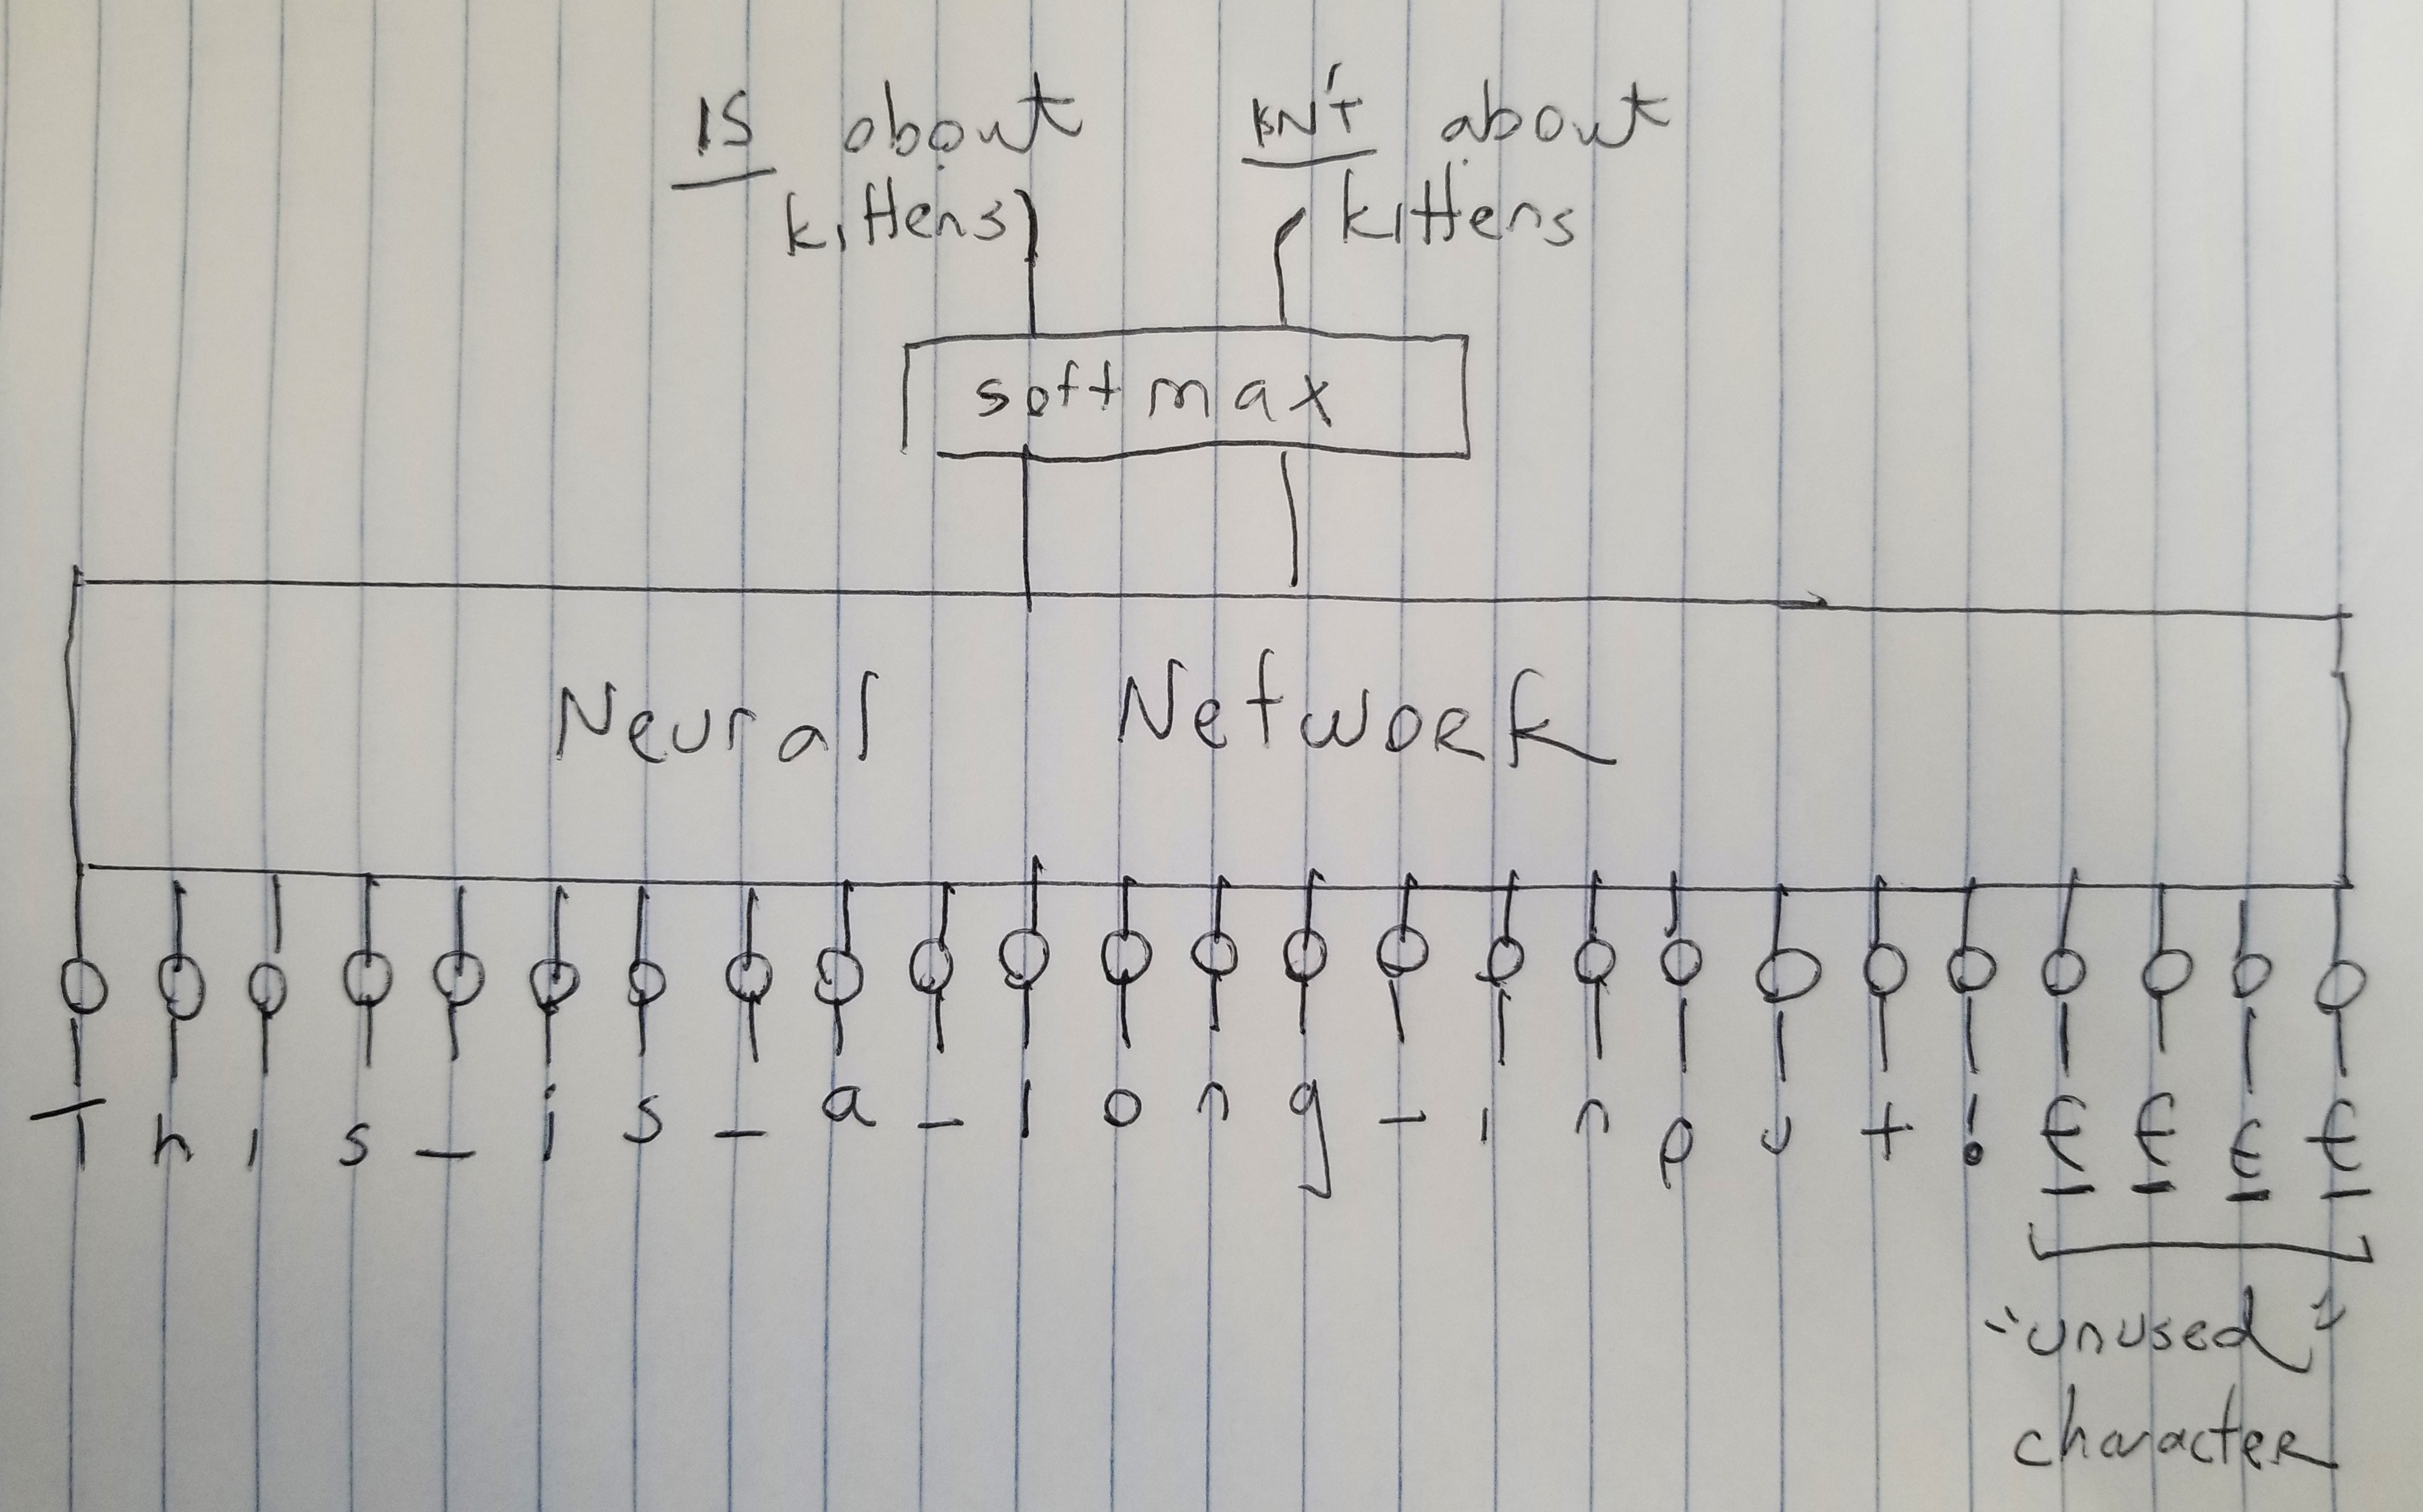
\includegraphics[width=0.7\textwidth]{lectRNN/wide_net.jpg}
\end{frame}
%***********************************************************
\begin{frame}{Issues with Standard idea}

\begin{itemize}
	\item High model complexity
	\begin{itemize}
	\item Max $n$ input tokens
	\item Size $m$ first hidden layer
	\item Means $n \times m$ weights to learn
	$$10^4 \times 10^5 = 10^9 = 1\text{B weights}$$
	\item[?] What if max tokens is 100K, average is 1000?
	\end{itemize}
\end{itemize}
\end{frame}
%***********************************************************
\begin{frame}{Issues}

\begin{itemize}
	\item High model complexity
	\begin{itemize}
	\item Max $n$ input tokens
	\item Size $m$ first hidden layer
	\item Means $n \times m$ weights to learn
	\item What if max tokens is 100K, average is 1000?
	\begin{itemize}
	\item We are spending effort learning a network that is too big
	\item Not much training data for right-most inputs
	\end{itemize}
	\item[?] What other issues are there? 
	\end{itemize}
\end{itemize}
\end{frame}
%***********************************************************
\begin{frame}{Issues}

\begin{itemize}
	\item High model complexity
	\begin{itemize}
	\item Max $n$ input tokens
	\item Size $m$ first hidden layer
	\item Means $n \times m$ weights to learn
	\item What if max tokens is 100K, average is 1000?
	\begin{itemize}
	\item We are spending effort learning a network that is too big
	\item Not much training data for right-most inputs
	\end{itemize}
	\item[?] What other issues are there? 
	\begin{itemize}
	\item We can't handle bigger lengths
	\item We have to use all the inputs
	\item Words positions are considered equivalent
	\end{itemize}
	\end{itemize}
\end{itemize}
\end{frame}
%***********************************************************
\begin{frame}{Words Position Issues}

\begin{itemize}
	\item Position $i$ treated as different from position $j$
	\begin{itemize}
	\item Not always the case!
	\item If we see ``kitten'' at pos 34 or pos 1034, it is perhaps the same
	\item We want to recognize pattern ``kitten'' regardless of position
	\item Or consider swapping the order of 2 paragraphs on Wikipedia. No one would notice!
	\end{itemize}
\end{itemize}
\end{frame}
%***********************************************************
\begin{frame}{So Idea Is To Allow Recursive Links}

\begin{columns}
\begin{column}{0.6\textwidth}
\begin{itemize}
	\item Results in an RNN
	\item Classic RNN is Elman Network
	\item The output from the hidden layer is pushed to the output AND copied to the state layer
	\item Input from context neurons is fed in with the input data
	\item There are NO weights from the neurons output to the states
	\item There ARE weights from the states  to the neuron inputs
\end{itemize}
\end{column}
\begin{column}{0.4\textwidth}
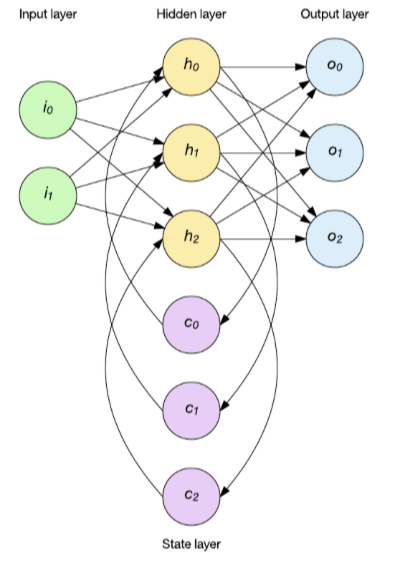
\includegraphics[width=1\textwidth]{lectRNN/Elman.png}
\end{column}
\end{columns}
\end{frame}
%***********************************************************
\begin{frame}[fragile]{Elman Network}

\begin{itemize}
	\item Have a set of context nodes (the "state layer") (``c'' neurons in previous slide)
	\item They read value of the hidden layer
	\begin{itemize}
		\item Non-trainable (e.g. values are not transformed)
		\item Value simply remembered for one time tick 
	\end{itemize}
	\item To process $t$ ticks  of data:
\end{itemize}

\begin{SQL}
init state layer to zeros
for i = 1 to $t$
  read input $x_i$
  $x_i$ along with state layer used to update hidden layer
  if ($i == t$) // for sequence-to-sequence, omit "if clause"
    hidden layer used to produce output
  hidden layer copied to state layer
end for 
\end{SQL}
\end{frame}
%***********************************************************
\begin{frame}{Sequence-to-Sequence?}

\begin{itemize}
	\item Input is a sequence
	\item Output is a sequence
	\item Output is generated at each time tick
	\item Lengths do not have to be identical
	\item Examples
	\begin{itemize}
		\item Machine translation
		\item Creating captions for video 
		\item Questions and answers
	\end{itemize}
\end{itemize}
\end{frame}

%***********************************************************
\begin{frame}[fragile]{Elman Network in Practice}

\begin{columns}
\begin{column}{0.6\textwidth}
\begin{itemize}
	\item Concatenate $x_i$ and the state values
	\item Perform the matrix multiplication to get the inputs to the next layer
	\item At the top, use only the hidden layer to product the output
\end{itemize}
\end{column}
\begin{column}{0.4\textwidth}
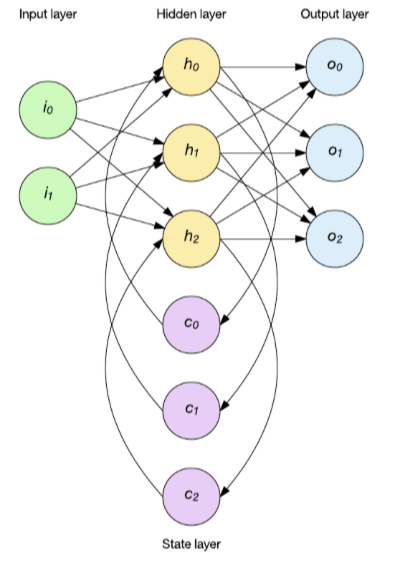
\includegraphics[width=1\textwidth]{lectRNN/Elman.png}
\end{column}
\end{columns}
\end{frame}

%***********************************************************
\begin{frame}{Elman Network}

\begin{itemize}
	\item We can have many hidden layers
	\item That is, a ``deep net''
	\item In this case
	\begin{itemize}
		\item Last hidden layer output copied to state
		\item State used as input to first hidden layer...
		\item In next time tick
	\end{itemize}
\end{itemize}
\end{frame}
%***********************************************************
\begin{frame}{Jordan Network}

\begin{columns}
\begin{column}{0.6\textwidth}
\begin{itemize} 
	\item Similar, but copy output values, not hidden values
	\item Can be used for sequence-to-sequence
	\item Must be producing output at each tick
\end{itemize}
\end{column}
\begin{column}{0.4\textwidth}
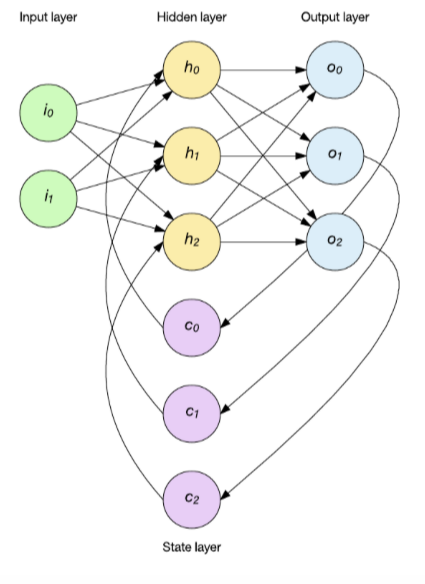
\includegraphics[width=1\textwidth]{lectRNN/Jordan.png}
\end{column}
\end{columns}
\end{frame}
%***********************************************************
\begin{frame}{Training}

\begin{itemize}
        \item Classic algorithm is back-propagation through time
	\item That is, view RNN as compact representation for a complex graph
	\item Unroll the complex graph
	\item And then use back-propagation on that
	\begin{itemize}
		\item Key difference from classic back-propagation:
		\item Weights are constrained to repeat
		% since you are learning one set of weights, but basically unrolling the network, it appears to be possible to have > 1 set of weights, but it's not
	\end{itemize}
\end{itemize}
\end{frame}
%***********************************************************
\begin{frame}{Example: Unrolling an Elman Network}

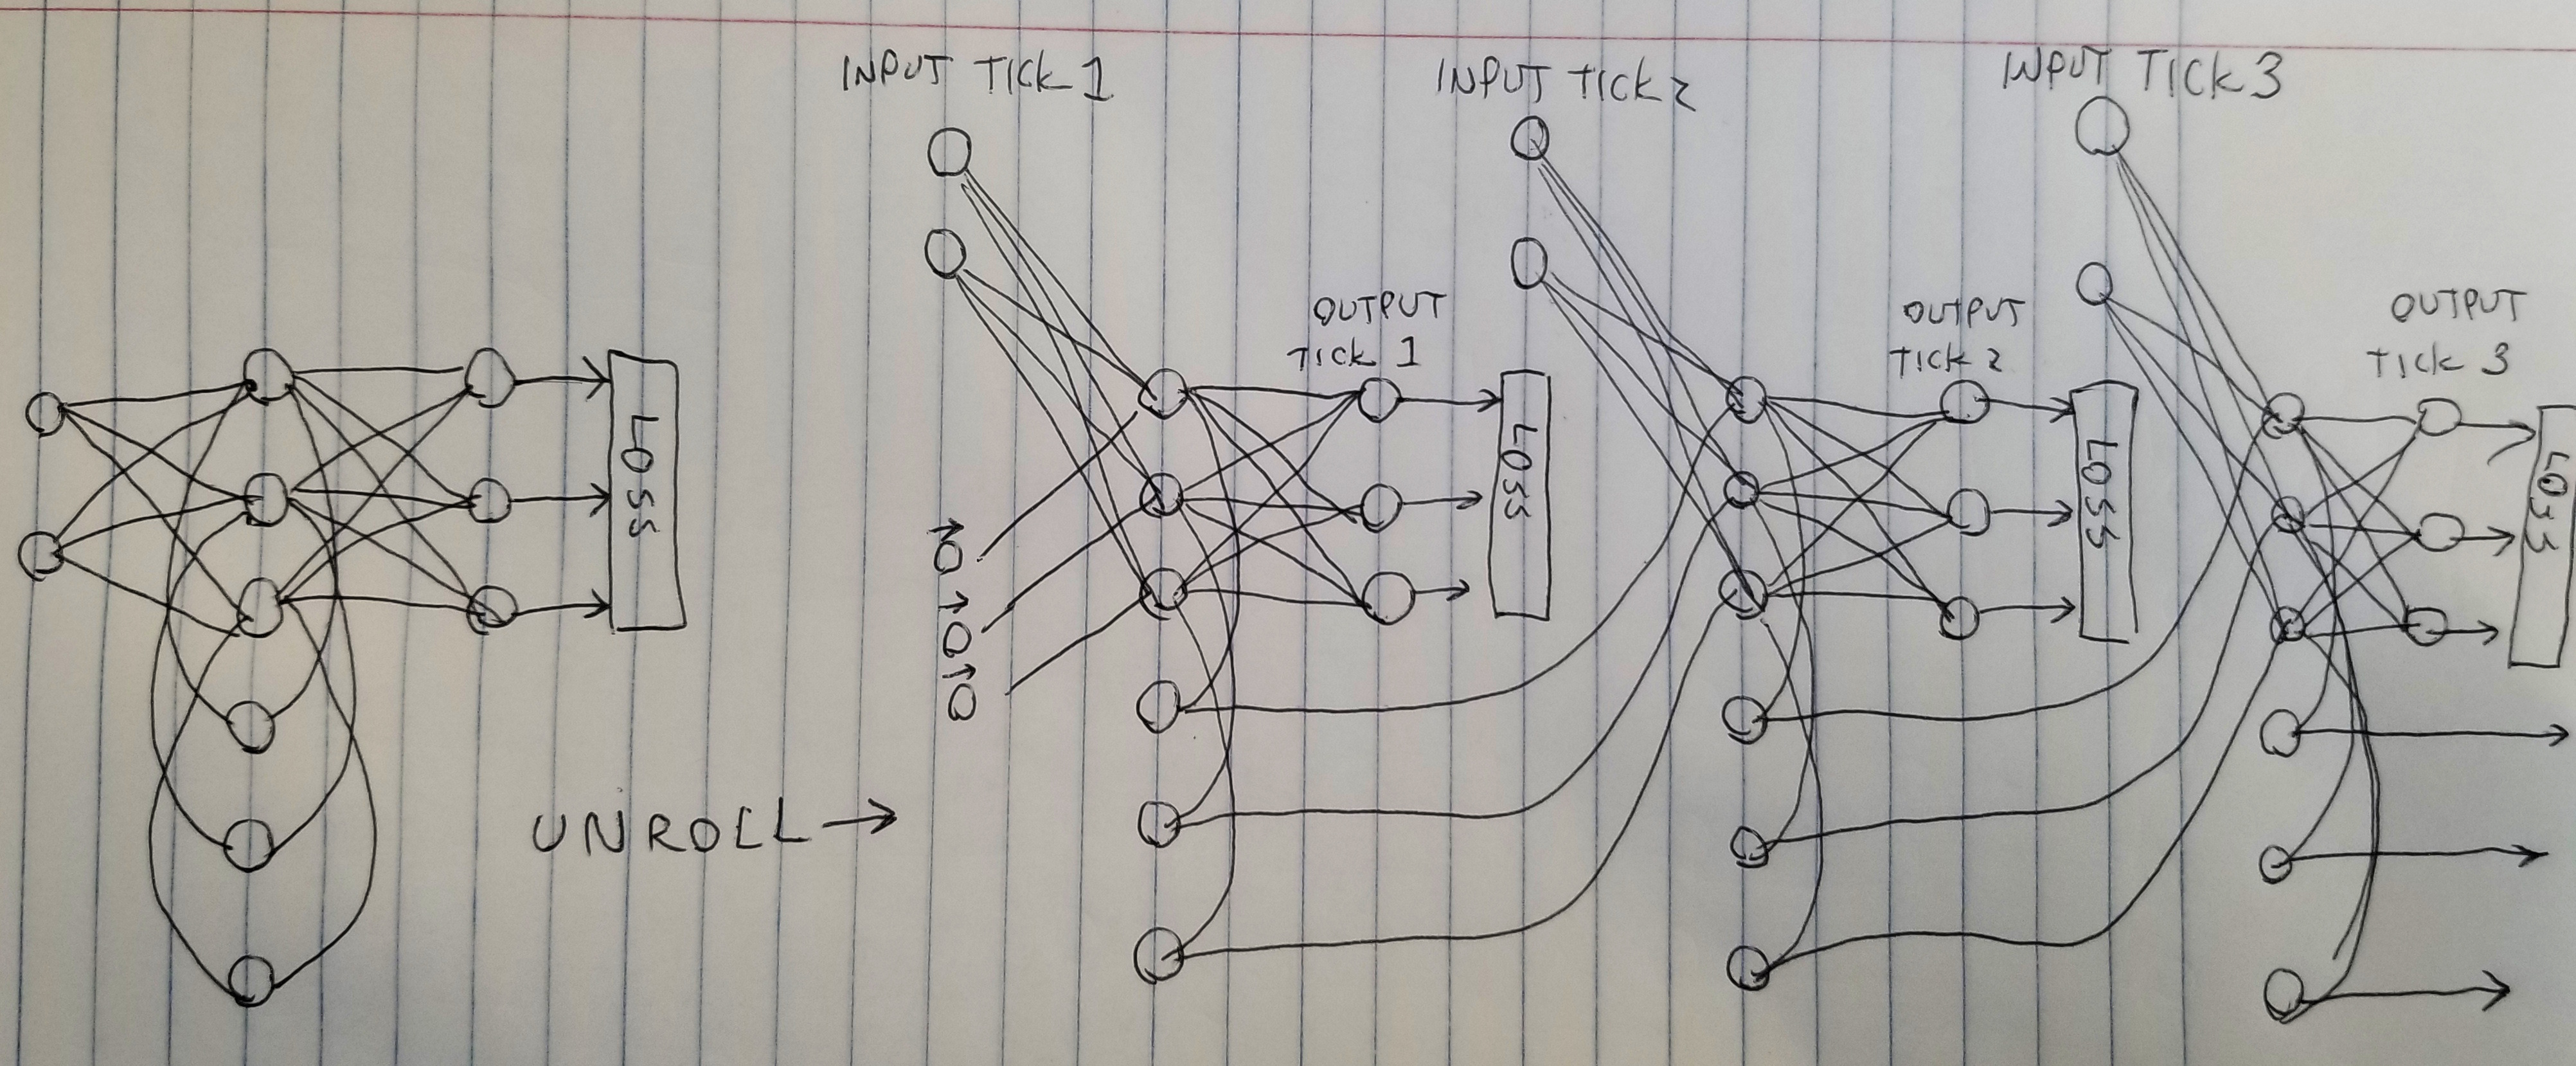
\includegraphics[width=0.85\textwidth]{lectRNN/Unrolled.jpg}

\begin{itemize}
	\item Example of unrolling a network for three time ticks
	\item Note distance backpropped error from last time tick must travel
	\begin{itemize}
		\item Goes through output neurons at time tick 3
		\item Through hidden neurons time tick 3
		\item Through hidden neurons time tick 2
		\item Through hidden neurons time tick 1
	\end{itemize}
\end{itemize}
\end{frame}
%***********************************************************
\begin{frame}{Training Difficulty: Vanishing Gradient}

\begin{itemize}
	\item Errors fall off exponentially as backpropped thru layers	
	\begin{itemize}
		\item Problem is that derivative of loss wrt activation function often $<< 1$
		\item Repeatedly multiplying causes backpropped errors to tend to zero
		\item Happens with deep, feed-forward nets, too 
		\item But unrolled RNNs are often especially deep
	\end{itemize}
\end{itemize}

\end{frame}
%***********************************************************
\begin{frame}{Training Difficulty: Vanishing Gradient}

\begin{itemize}
	\item Errors fall off exponentially as backpropped thru layers	
	\begin{itemize}
		\item Problem is that derivative of loss wrt activation function often $<< 1$
		\item Repeatedly multiplying causes backpropped errors to tend to zero
		\item Happens with deep, feed-forward nets, too 
		\item But unrolled RNNs are often especially deep
	\end{itemize}
	\item Means that in a deep net...
	\begin{itemize}
	\item ...backprop does not affect weights in first (leftmost) few layers
	\end{itemize}
\end{itemize}

\end{frame}
%***********************************************************
\begin{frame}{Training Difficulty: Vanishing Gradient}

\begin{itemize}
	\item Especially a problem if there is just one output at end of unrolled RNN
	\item Like in a pure classification task
	\begin{itemize}
	\item Means that you will learn to classify
	\item ...using only the last few time-tick's worth of data
	\item Because early data can't interact with backpropped error
	\end{itemize}
\end{itemize}

\end{frame}
%***********************************************************
\begin{frame}{Other Issues with RNNs}

\begin{itemize}
	\item Very expensive to train
	\item Still expensive to use
\end{itemize}

\end{frame}
%***********************************************************
\begin{frame}{LSTMs}

\begin{itemize} 
	\item Long Short Term Memory networks
	\begin{itemize}
	\item Special RNN designed to deal with vanishing gradient problem
	\item In LSTM, long term memory is not pushed through activation functions
	\item So we don't have vanishing gradients
	\item Will discuss next time!
	\end{itemize}
\end{itemize}
\end{frame}
%***********************************************************

\begin{frame}{Questions?}
\end{frame}
\end{document}
